\documentclass{article}
\usepackage{tikz}
\usetikzlibrary{trees}

\begin{document}
	
	\title{Simple Tree Diagram or Hierarchical Structure in the Document with appropriate Labels using the TikZ Library}
	\date{}
	\maketitle
	
	\begin{center}
		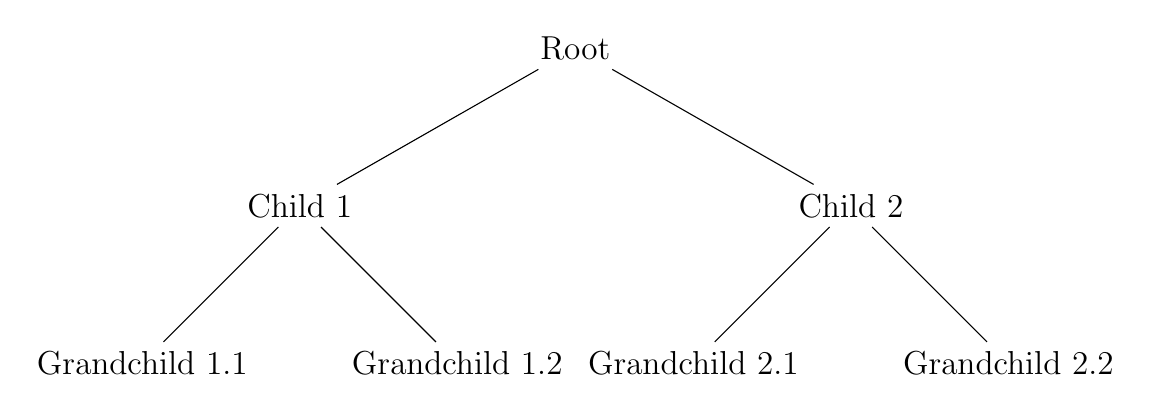
\begin{tikzpicture}[
			level 1/.style={sibling distance=7cm},
			level 2/.style={sibling distance=4cm},
			level distance=2cm,
			every node/.style={font=\large} % Increase font size here (e.g. \large, \Large)
			]
			\node {Root}
			child { node {Child 1} 
				child { node {Grandchild 1.1} }
				child { node {Grandchild 1.2} }
			}
			child { node {Child 2} 
				child { node {Grandchild 2.1} }
				child { node {Grandchild 2.2} }
			};
		\end{tikzpicture}
	\end{center}
	
\end{document}
